\section[Задача Коши, условная аппроксимация, альфа-устойчивость, модельные схемы]{Задача Коши,
  условия аппроксимации $p$-го порядка на решении, \\
  $\alpha$-устойчивость. Модельные схемы.}

\begin{definition}
  Задачей Коши первого порядка называют следующую дифференциальную
  задачу
  \[\begin{cases}
      y'(x) = f(y(x),x),\ y\in C^{(m)}[x_0,x_0+X],\ \norm{y}=\max_{x\in[x_0,x_0+X]}\abs{y(x)} \\
      y(x_0) = y^0
    \end{cases}\]
  Для такой задачи предлагается строить следующую разностную схему
  \begin{equation}\label{eq:cauchy:recur_scheme}
    \begin{array}{c}
      h=\frac{X}{N},\ x_i=x_o+i\cdot h,\ y_h=\{y_i\}_{i=0}^{N},\ \norm{y_h}_{Y_h}=\max_{i}\abs{y_k} \\
      \begin{cases}
        \frac{1}{h}\sum\limits_{i=0}^na_{-i}y_{k-i}=\sum\limits_{i=0}^nb_{-i}f(y_{k-i},x_{k-i}) \\
        y_0,y_1,\ldots,y_{n-1} - \text{ начальные условия (может быть больше одного)}
      \end{cases}                                                                     \\
    \end{array}
  \end{equation}
  Если $a_0\neq0,\ b_0\neq0$, то схема называется неявной,
  если $a_0\neq0,\ b_0=0$, то явной,
  а если $a_0=0,\ b_0\neq0$ с забеганием вперед.
\end{definition}

Хотим для такой разностной схемы проверять условие аппроксимации на решении,
чтобы далее пользоваться теоремой Филиппова.

Зададим функцию погрешности
\[r^k_h\defeq\frac{1}{h}\sum_{i=0}^na_{-i}y(x_{k-i})-\sum_{i=0}^nb_{-i}f(y(x_{k-i}),x_{k-i})\]

Условия аппроксимации на решении с порядком $p$ на отрезке $[x_0,x_0+X]$:
$\begin{cases}\norm{r_h}_{F_h}\leq ch^p \\
    \norm{f_h-(f)_h}_{F_h}\underset{h\rightarrow0}{\rightarrow}0
  \end{cases}$

Коэффициенты в общем случае $a_{-i}$ и $b_{-i}$ находятся из условий
аппроксимации на задаче $\norm{L_h(y)_{Y_h} - (Ly)_{F_h}}_{F_h}+\norm{(f)_{F_h}-f_h}_{F_h}\leq c_1h^{p_1}$.

\begin{remark}
  Так как задача Коши по сути сводится к интегрированию $f$, то
  рассуждения о погрешности формул численного дифференицирования здесь неприменимы.
\end{remark}

\begin{remark}
  Есть определенные методы построения краевых условий (например, $\delta$-поправка),
  которые повышают порядок сходимости, но в лекционном материале они не рассматриваются.
\end{remark}

\begin{theorem}[Условия аппроксимации $p$-го порядка на решении]
  Для задачи $y'(x)=f(x)$ с разностной схемой \eqref{eq:cauchy:recur_scheme}
  условия аппроксимации $p$-го порядка на решении имеют вид
  \[\sum_{i=0}^na_{-i}=0;\ \sum_{i=0}^nb_{-i}=1;\ \sum_{i=0}^na_{-i}i=-1;\]
  \[\sum_{i=0}^n(a_{-i}i+b_{-i}s)i^{s-1}=0,\ s=2,\ldots,p\]
\end{theorem}
\begin{proof}
  \begin{enumerate}
    \item Проверим условие нормировки правых частей
          \[\norm{f_h-(f)_h}_{F_h}=\norm{f(x_{k-i})-\sum_{i=0}^nb_{-i}f(x_{k-i})}_{F_h}=\norm{f(x_{k-i})\left(1-\sum_{i=0}^nb_{-i}\right)}_{F_h}\underset{h\rightarrow0}{\rightarrow}0\Leftrightarrow\sum_{i=0}^nb_{-i}=1\]
    \item Выпишем ряд Тейлора для левой и правой части в узлах $\{x_k\}$:
          \begin{align*}
            y(x_k-ih)=y(x_k)-hy'(x_k)+\sum_{s=2}^{p}\frac{(-ih)^{s}y^{(s)}(x_k)}{s!} + \bigO(h^{p+1})        \\
            f(x_k-ih)=y'(x_k-ih)=y'(x_k)+\sum_{s=2}^{p}\frac{(-ih)^{s-1}y^{(s)}(x_k)}{(s-1)!} + \bigO(h^{p}) \\
          \end{align*}
          Запишем условие аппроксимации на решении до $p$-го порядка:
          \begin{multline*}
            \abs{\frac{1}{h}\sum_{i=0}^na_{-i}y(x_k-ih)-\sum_{i=0}^nb_{-i}f(x_k-ih)} =
            = \left|\frac{1}{h}\sum_{i=0}^na_{-i}y(x_k)+\frac{1}{h}\sum_{i=0}^na_{-i}(-ihy'(x_k))-\sum_{i=0}^nb_{-i}y'(x_k)\right.+ \\
            +\left.\frac{1}{h}\sum_{i=0}^na_{-i}\sum_{s=2}^{p}\frac{(-ih)^sy^{(s)}(x_k)}{s!}-\sum_{i=0}^nb_{-i}\sum_{s=2}^{p}\frac{(-ih)^{s-1}y^{(s)}(x_k)}{(s-1)!}\right|=
          \end{multline*}
          \[
            =\left|\frac{y(x_k)}{h}\sum_{i=0}^na_{-i}+y'(x_k)\left(-\sum_{i=0}^na_{-i}i-\sum_{i=0}^nb_{-i}\right)
            +\sum_{s=2}^{p}\frac{(-h)^{s-1}y^{(s)}}{s!}\left(\sum_{i=0}^n(a_{-i}i+b_{-i}s)i^{s-1}\right)\right|\leq ch^p
          \]
          Для выполнения условия аппроксимации нужно, чтобы все коэффициенты до $h^p$ занулились, отсюда
          и из проверки нормировки следует доказательство теоремы.
  \end{enumerate}
\end{proof}
\begin{remark}
  Для уверенности, что схема аппроксимирует (т.е. $p = 1$)
  необходимо и достаточно проверить первые три уравнения.

  Для того, чтобы найти $a_{-i}$ и $b_{-i}$ надо решить систему уравнений.
  Для того, чтобы система была разрешима, важно проверить $p=2n$.
\end{remark}
\begin{example}
  Схемы Адамса со вторым порядком аппроксимации на решении:
  \[\begin{array}{ccc}
      \text{явная схема}:  & \frac{y_{k}-y_{k-1}}{h} = & \frac{3}{2}f_{k-1}-\frac{1}{2}f_{k-2}   \\
      \text{неявня схема}: & \frac{y_{k}-y_{k-1}}{h} = & \frac{1}{2}\left({f_{k}+f_{k-1}}\right)
    \end{array}\]
\end{example}

Устойчивость разностных схем для задач Коши довольно
затруднительно проверить по определению, используют более слабое понятие
$\alpha$-устойчивости.

\begin{definition}
  Разностная схема $\frac{1}{h}\sum_{i=0}^{n}a_{-i}y_{k-i}=fk$ для задачи
  $y'(x)=f(x)$ называется $\alpha$-устойчивой, если все корни
  соответствующего характеристического многочлена однородного
  разностного уравнения принадлежат единичному кругу и на границе
  нет кратных корней.
\end{definition}

\begin{remark}
  $\alpha$-устойчивость строго говоря не связана с устойчивостью, но
  для широкого класса задач обеспечивает сходимость.
  Рассмотрим схемы с $\alpha$-устойчивостью, но с разными
  результатами.
  \begin{example}
    Будем численно решать задачу Коши $y'=-y,\ y(0)=1,\ x=[0,X]$
    с точным решением $y(x)=e^{-x}$. Проверим разные разностные схемы и
    и оценим их качество.
    \begin{enumerate}
      \item Неявная схема Адамса: $n=1,\ p=2$
            \[
              \begin{cases}
                \frac{y_{k}-y_{k-1}}{h}=\frac{1}{2}\left({f_{k}+f_{k-1}}\right) \\
                y_0=y^0
              \end{cases} \Leftrightarrow
              \begin{array}{c}
                x_k=x_0+ih,\ h=\frac{X}{n}                            \\
                ((y)_{Y_n})_k=y(x_k)=:y_k                             \\
                f(y_{k},x_k)=-y_k=:f_{k}                              \\
                ((f)_{F_n})_k=\frac{1}{2}\left({f_{k}+f_{k-1}}\right) \\
              \end{array}\Leftrightarrow
              \begin{cases}
                \frac{y_k-y_{k-1}}{h}=-\frac{y_k+y_{k-1}}{2} \\
                y_0=1
              \end{cases}
            \]
            Проверим условие аппроксимации второго порядка:
            \[\begin{array}{c}
                \sum\limits_{i=0}^na_{-i}=1-1=0;\ \sum\limits_{i=0}^nb_{-i}=\frac{1+1}{2}=1;\ \sum\limits_{i=0}^na_{-i}i=1\cdot0 - 1\cdot1=-1 \\
                \sum\limits_{i=0}^n(a_{-i}i+b_{-i}\cdot2)i^{2-1}=-1 + \frac{1}{2}\cdot2=0
              \end{array}\]

            Проверим $\alpha$-устойчивость: $y_k-y_{k-1}=0\Rightarrow P(\mu)=\mu-1=0\Rightarrow\mu=1$

            Таким образом разностная схема должна сходиться.
            Мы можем проверить это проверить, решив эквивалентное однородное
            разностное уравнение с постоянными коэффициентами:
            \[\frac{y_k-y_{k-1}}{h}=-\frac{y_k+y_{k-1}}{2}\Leftrightarrow y_k(2-h)+y_{k-1}(2+h)=0;\ P(\mu)=0\Rightarrow\mu=\frac{1-h/2}{1+h/2}\Rightarrow y_k=\left(\frac{1-h/2}{1+h/2}\right)^k\]
            \[y_n=\left(\frac{1-h/2}{1+h/2}\right)^{X/h}\overunderset{\text{Тейлор в 0}}{h\rightarrow0}{\longrightarrow}\left(1-h+\bigO(h^2)\right)^{X/h}\underset{\text{2й замечательный}}{\longrightarrow}e^{-X}=y(x_n)\]
            \begin{figure}[ht]
              \centering
              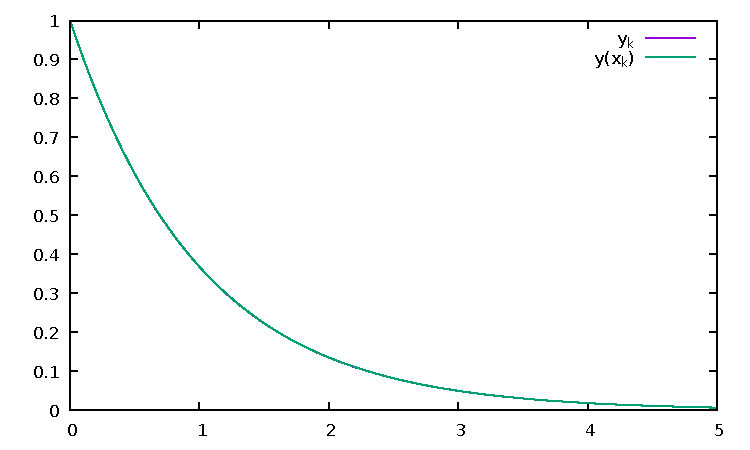
\includegraphics[scale=0.6]{12/1Scheme.pdf}
              \caption{Численные значения при $X=5$, $n=100$}
            \end{figure}
            \newpage
      \item Вторая схема аппроксимации
            \[
              \begin{array}{c}
                ((y)_{Y_n})_k=y(x_k)=:y_k         \\
                ((f)_{F_n})_k=f_k:=f(x_k)=-y(x_k) \\
              \end{array}\Rightarrow
              \begin{cases}
                \frac{y_{k+1}-y_{k-1}}{2h}+y_k=0 \\
                y_0=1,\ y_1=1-h
              \end{cases}
            \]
            \begin{enumerate}
              \item Аппроксимацию второго порядка на решении можно проверить, используя теорему выше, но
                    для разнообразия проверим по определению
                    \begin{multline*}
                      \norm{L_h(y)_{Y_h}-f_h}_{F_h}=\max_{k}\left|\frac{y(x_k+h)-y(x_k-h)}{2h}-f(x_k)\right|=\\
                      \left|\begin{array}{c}
                        y(x_k\pm h)=y(x_k)\pm y'(x_k)h + y''(x_k)\frac{h^2}{2}\pm y'''(x_k)\frac{h^3}{6}+\bigO(h^4) \\
                        f(x_k)=y'(x_k) \text{ -- по условию}
                      \end{array}\right| \\
                      =\max_{k}\left|\frac{2hy'(x_k)+\bigO(h^3)}{2h}-y'(x_k)\right| \leq ch^2
                    \end{multline*}
              \item Проверим аппроксимацию на краях $\norm{l_h(y)_h-\varphi_h}_{\Phi_h}$
                    \begin{flalign*}
                      & |y(0)-y_0|=0\leq ch^2 \\
                      & |y(h)-y_1|=|\overbrace{y(0)}^{=1}+y'(0)h+\bigO(h^2)-1+h|=|h\overbrace{(y'(0)+y(0))}^{=0}+\bigO(h^2)|=\leq ch^2
                    \end{flalign*}
              \item Проверим условие нормировки: $\norm{(f)_h-f_h}_{F_h}=|f(x_k)-f(x)|\rightarrow0$
            \end{enumerate}
            Разностная схема имеет второй порядок аппроксимации.
            \[\frac{y_{k+1}-y_{k-1}}{2h}=0\Rightarrow P(\mu)=\mu^2-1\Rightarrow \mu=\pm 1\]
            Схема $\alpha$-устойчива.

            Судя по всей той теории, что описана выше, так как есть $\alpha$-устойчивость, то
            такую разностную схему можно применять для численного подсчета. Давайте попробуем посчитать
            иначе: в разностной схеме -- разностное уравнение второго порядка с постоянными коэффициентами.
            \[\frac{y_{k+1}-y_{k-1}}{2h}+y_k=0\Rightarrow P(\mu)=\frac{\mu^2-1}{2h}+\mu=0\Rightarrow\mu_{1,2}=-h\pm\sqrt{1+h^2}\]
            \[y_k=C_1(-h+\sqrt{1+h^2})^k+C_2(\ \underbrace{-h-\sqrt{1+h^2}}_{<-1}\ )^k\]
            Обратим внимание, что из-за того, что второй корень по модулю больше единицы,
            при большом количестве шагов правое слагаемое в сумме будет доминировать, в результате
            чего решение разностной задачи будет болтаться в зависимости от четности $k$.
            То есть эту схему лучше не применять.
            \begin{figure}[h]
              \centering
              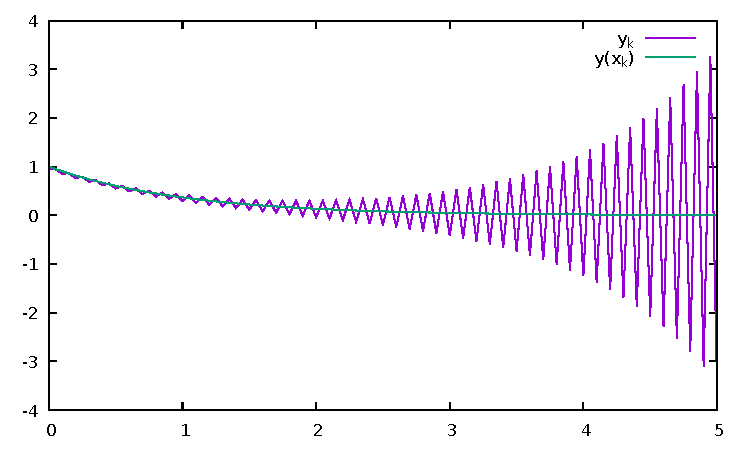
\includegraphics[scale=0.75]{12/2Scheme.pdf}
              \caption{Численные значения при $X=5$, $n=100$}
            \end{figure}
            \newpage
      \item Третья схема
            \[
              \begin{cases}
                \frac{y_{k+1}-y_{k-1}}{2h}=-\frac{y_{k+1}+y_{k-1}}{2} \\
                y_0=1,\ y_1=1-h                                       \\
              \end{cases}
            \]

            Аналогично предыщум пунктам проверяется аппроксимация на решении
            2 степени и $\alpha$-устойчивость. Решения разностного уравнения имеют вид
            \[\mu_{1,2}=\pm\sqrt{\frac{1-h}{1+h}},\ \abs{\mu_{1,2}}<1\]

            Заметим, что в данной схеме каждый следующий элемент порождается через предпоследний,
            из-за чего решение задачи будет менять знак в зависимости от $k$.
            По такой схеме можно считать, но в отличие от первой для нее нужно
            дополнительное краевое условие, которое мы получили зная итоговый ответ.
            В жизни же мы итоговый ответ не знаем.
            \begin{figure}[h]
              \centering
              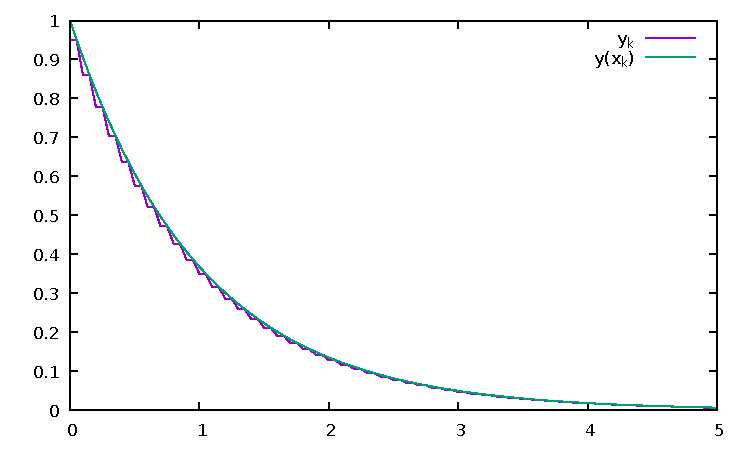
\includegraphics[scale=0.75]{12/3Scheme.pdf}
              \caption{Численные значения при $X=5$, $n=100$}
            \end{figure}
    \end{enumerate}
  \end{example}
\end{remark}
